\documentclass{lecture}

%\setbeameroption{show notes on second screen}
\usepackage{listliketab}
\usepackage{url}
\usepackage{xspace}
\usepackage{graphicx}
\usepackage{LI}
\usepackage{etex}
\usepackage{times}
\usepackage{booktabs}
\usepackage{color}
\usepackage{latexsym}
\usepackage{tipa}
%\usepackage{wasysym}
\usepackage{tipa}
\usepackage{tikz}
\usepackage{tikz-qtree}
%\usepackage{textpos}
%\usepackage{MnSymbol}
\usetikzlibrary{arrows,automata,calc,positioning,through}
%\usepackage{verbatim} % for comment blocks
%\usepackage{ulem} % for strikethrough (sout)
\usepackage{pifont}
%\usepackage{ucs}
\usepackage[utf8]{inputenc}
\usepackage[T1]{fontenc}
%\usepackage{pylistings}
\usepackage{amsmath}
\usepackage{multirow}


\usefonttheme{professionalfonts} % using non standard fonts for beamer
\usefonttheme{serif} % default family is serif
%\setmainfont{fourier}

\definecolor{darkgreen}{cmyk}{0.74,0.06,0.98,0.2}

\newcommand{\red}[1]{\textcolor{usydred}{#1}}
\newcommand{\green}[1]{\textcolor{darkgreen}{#1}}
\newcommand{\blue}[1]{\textcolor{usydblue}{#1}}
\newcommand{\gold}[1]{\textcolor{usydyellow}{#1}}

%\usepackage{beamerthemesplit}

%\usepackage{javalistings}
%\usepackage{cpplistings}
\beamertemplatenavigationsymbolsempty
%\setbeamertemplate{navigation symbols}{}
%\setbeamertemplate{bibliography item}[text]


\usepackage[style=authoryear]{biblatex}
\renewcommand*\bibopenparen{[}
\renewcommand*\bibcloseparen{]}
\addbibresource{slides.bib}

\title{A Practical Algorithm for Topic Modeling with Provable Guarantees}
\author[Vanush \& Kristy]{Sanjeev Arora\\
		Rong Ge\\
		Yoni Halpern\\
		David Mimno\\
		Ankur Moitra\\
		David Sontag\\
		Yihcen Wu\\
		Michael Zhu}
\institute[\textschwa-lab]{Presented by: Vanush Vaswani and Kristy Hughes}
\date{}

\begin{document}

% Optional if you want to show outlines to structure the talk.
\AtBeginSection[]
{
  \begin{frame}
    %\frametitle{Outline: \thesection}
    \tableofcontents[currentsection]
  \end{frame}
}

\titleslide

%-------------------------------------------------%
\section[Intro]{Introduction}

\begin{plain}{Information Overload}
\vspace{-2ex}
\begin{center}

\includegraphics[scale=0.6]{figs/messy}
\end{center}
\end{plain}

\begin{plain}{Effective Organisation}
\vspace{-4ex}
\begin{center}
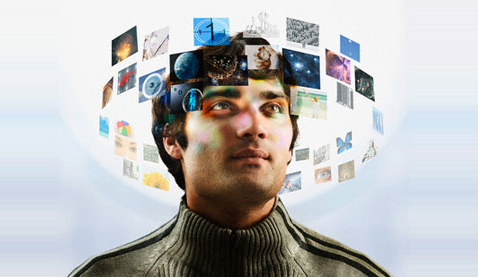
\includegraphics[scale=0.65]{figs/organised}
\end{center}
\end{plain}

\begin{plain}{Topics}
\vspace{-4ex}
\begin{center}
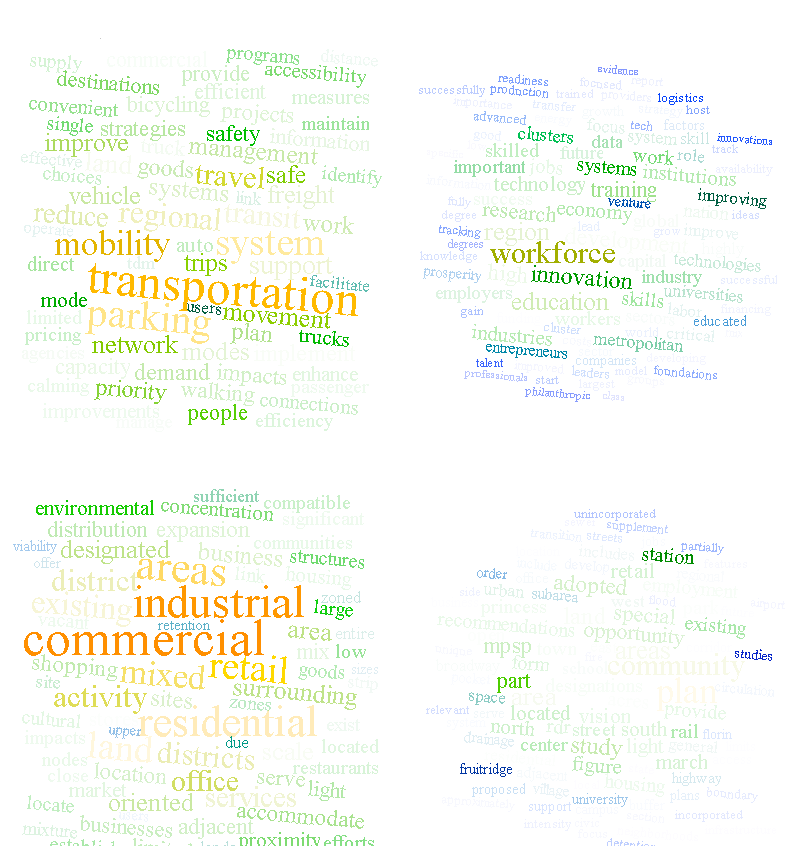
\includegraphics[scale=0.3]{figs/topic_visual}
\end{center}
\end{plain}

%-------------------------------------------------%
\section[Topic Models]{Topic Modelling}

\begin{plain}{Topics}
\begin{columns}
\column{0.3\textwidth}
\begin{center}
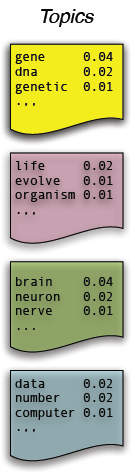
\includegraphics[scale=0.4]{figs/blei_topics}
\end{center}
\column{0.7\textwidth}
\begin{center}
Topics are distributions over words
\end{center}
\end{columns}
\end{plain}

\begin{plain}{Documents}
\begin{columns}
\column{0.3\textwidth}
\begin{center}
Documents have distribution of topics
\end{center}
\column{0.7\textwidth}
\begin{center}
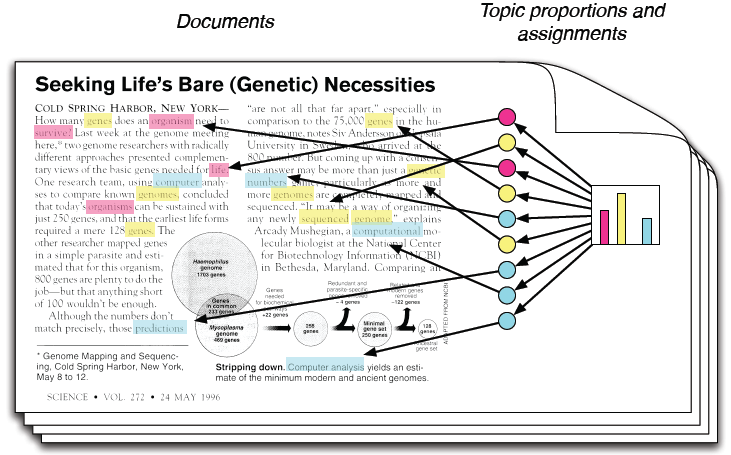
\includegraphics[scale=0.3]{figs/blei_docs}
\end{center}
\end{columns}
\end{plain}

\begin{plain}{Topic Modelling}
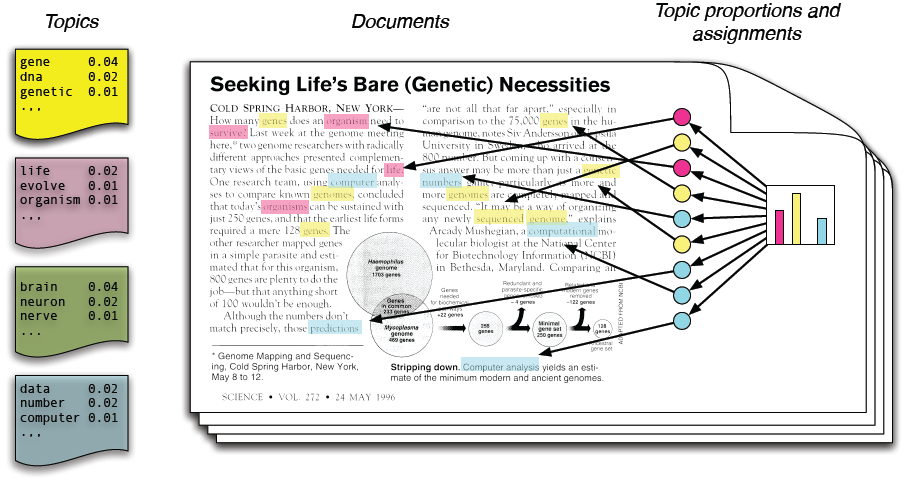
\includegraphics[scale=0.35]{figs/blei}
\end{plain}

\begin{plain}{Task}
\begin{itemize}
	\p Assume documents are generated by probabilistic model with unknown variables\\
	\p Infer hidden structure onto document\\
	\p Situate new document into model\\
\end{itemize}
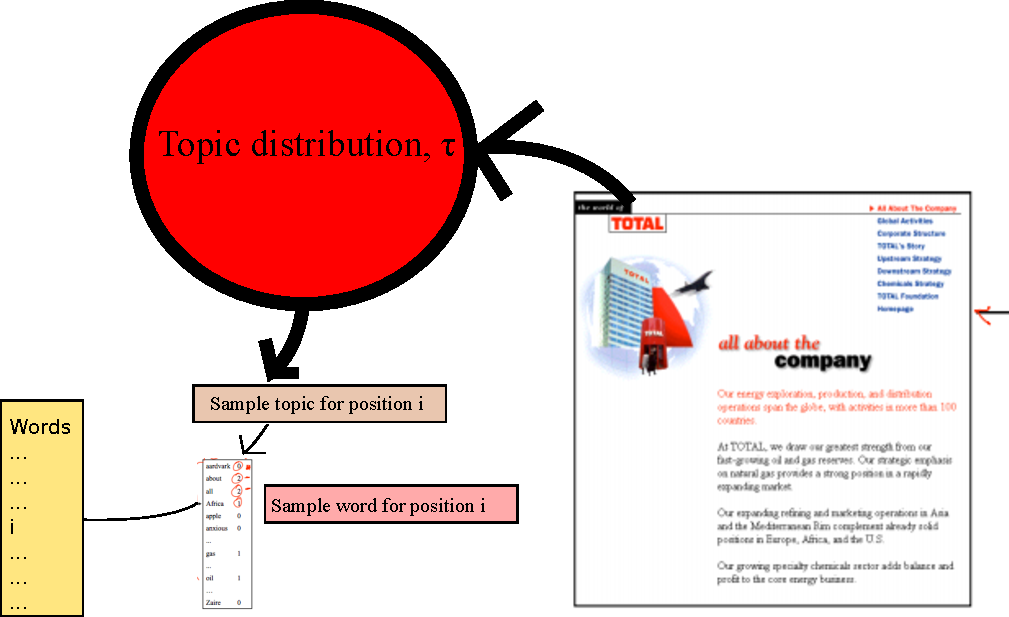
\includegraphics[scale=0.4]{figs/steps}
\end{plain}

\begin{plain}{Word-topic Matrix}
\begin{center}
\vspace{-2ex}
Extracted: Word-topic matrix
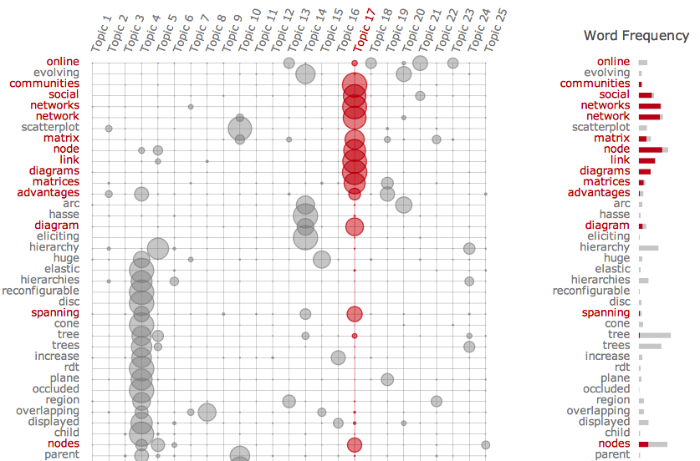
\includegraphics[scale=0.36]{figs/word_topic}\\
Aim: Find document-topic matrix
\end{center}
\end{plain}

\begin{plain}{Anchor Words}
\begin{itemize}
	\p Word-topic distributions are separable
	\p There is a word unique to each topic
	\p Indicates document is partially about that topic
	\p Can learn parameters in polynomial time provided there is a large enough number of documents
\end{itemize}
\end{plain}

\begin{plain}{Approximate Inference \& Provable Guarantees}
\begin{columns}
\column{0.55\textwidth}
\begin{itemize}
	\p Document-topic inference:
	\begin{itemize}
		\item NP-hard
	\end{itemize}	
	\p Approximate techniques
	\p Provably polynomial-time?
\end{itemize}
\column{0.55\textwidth}
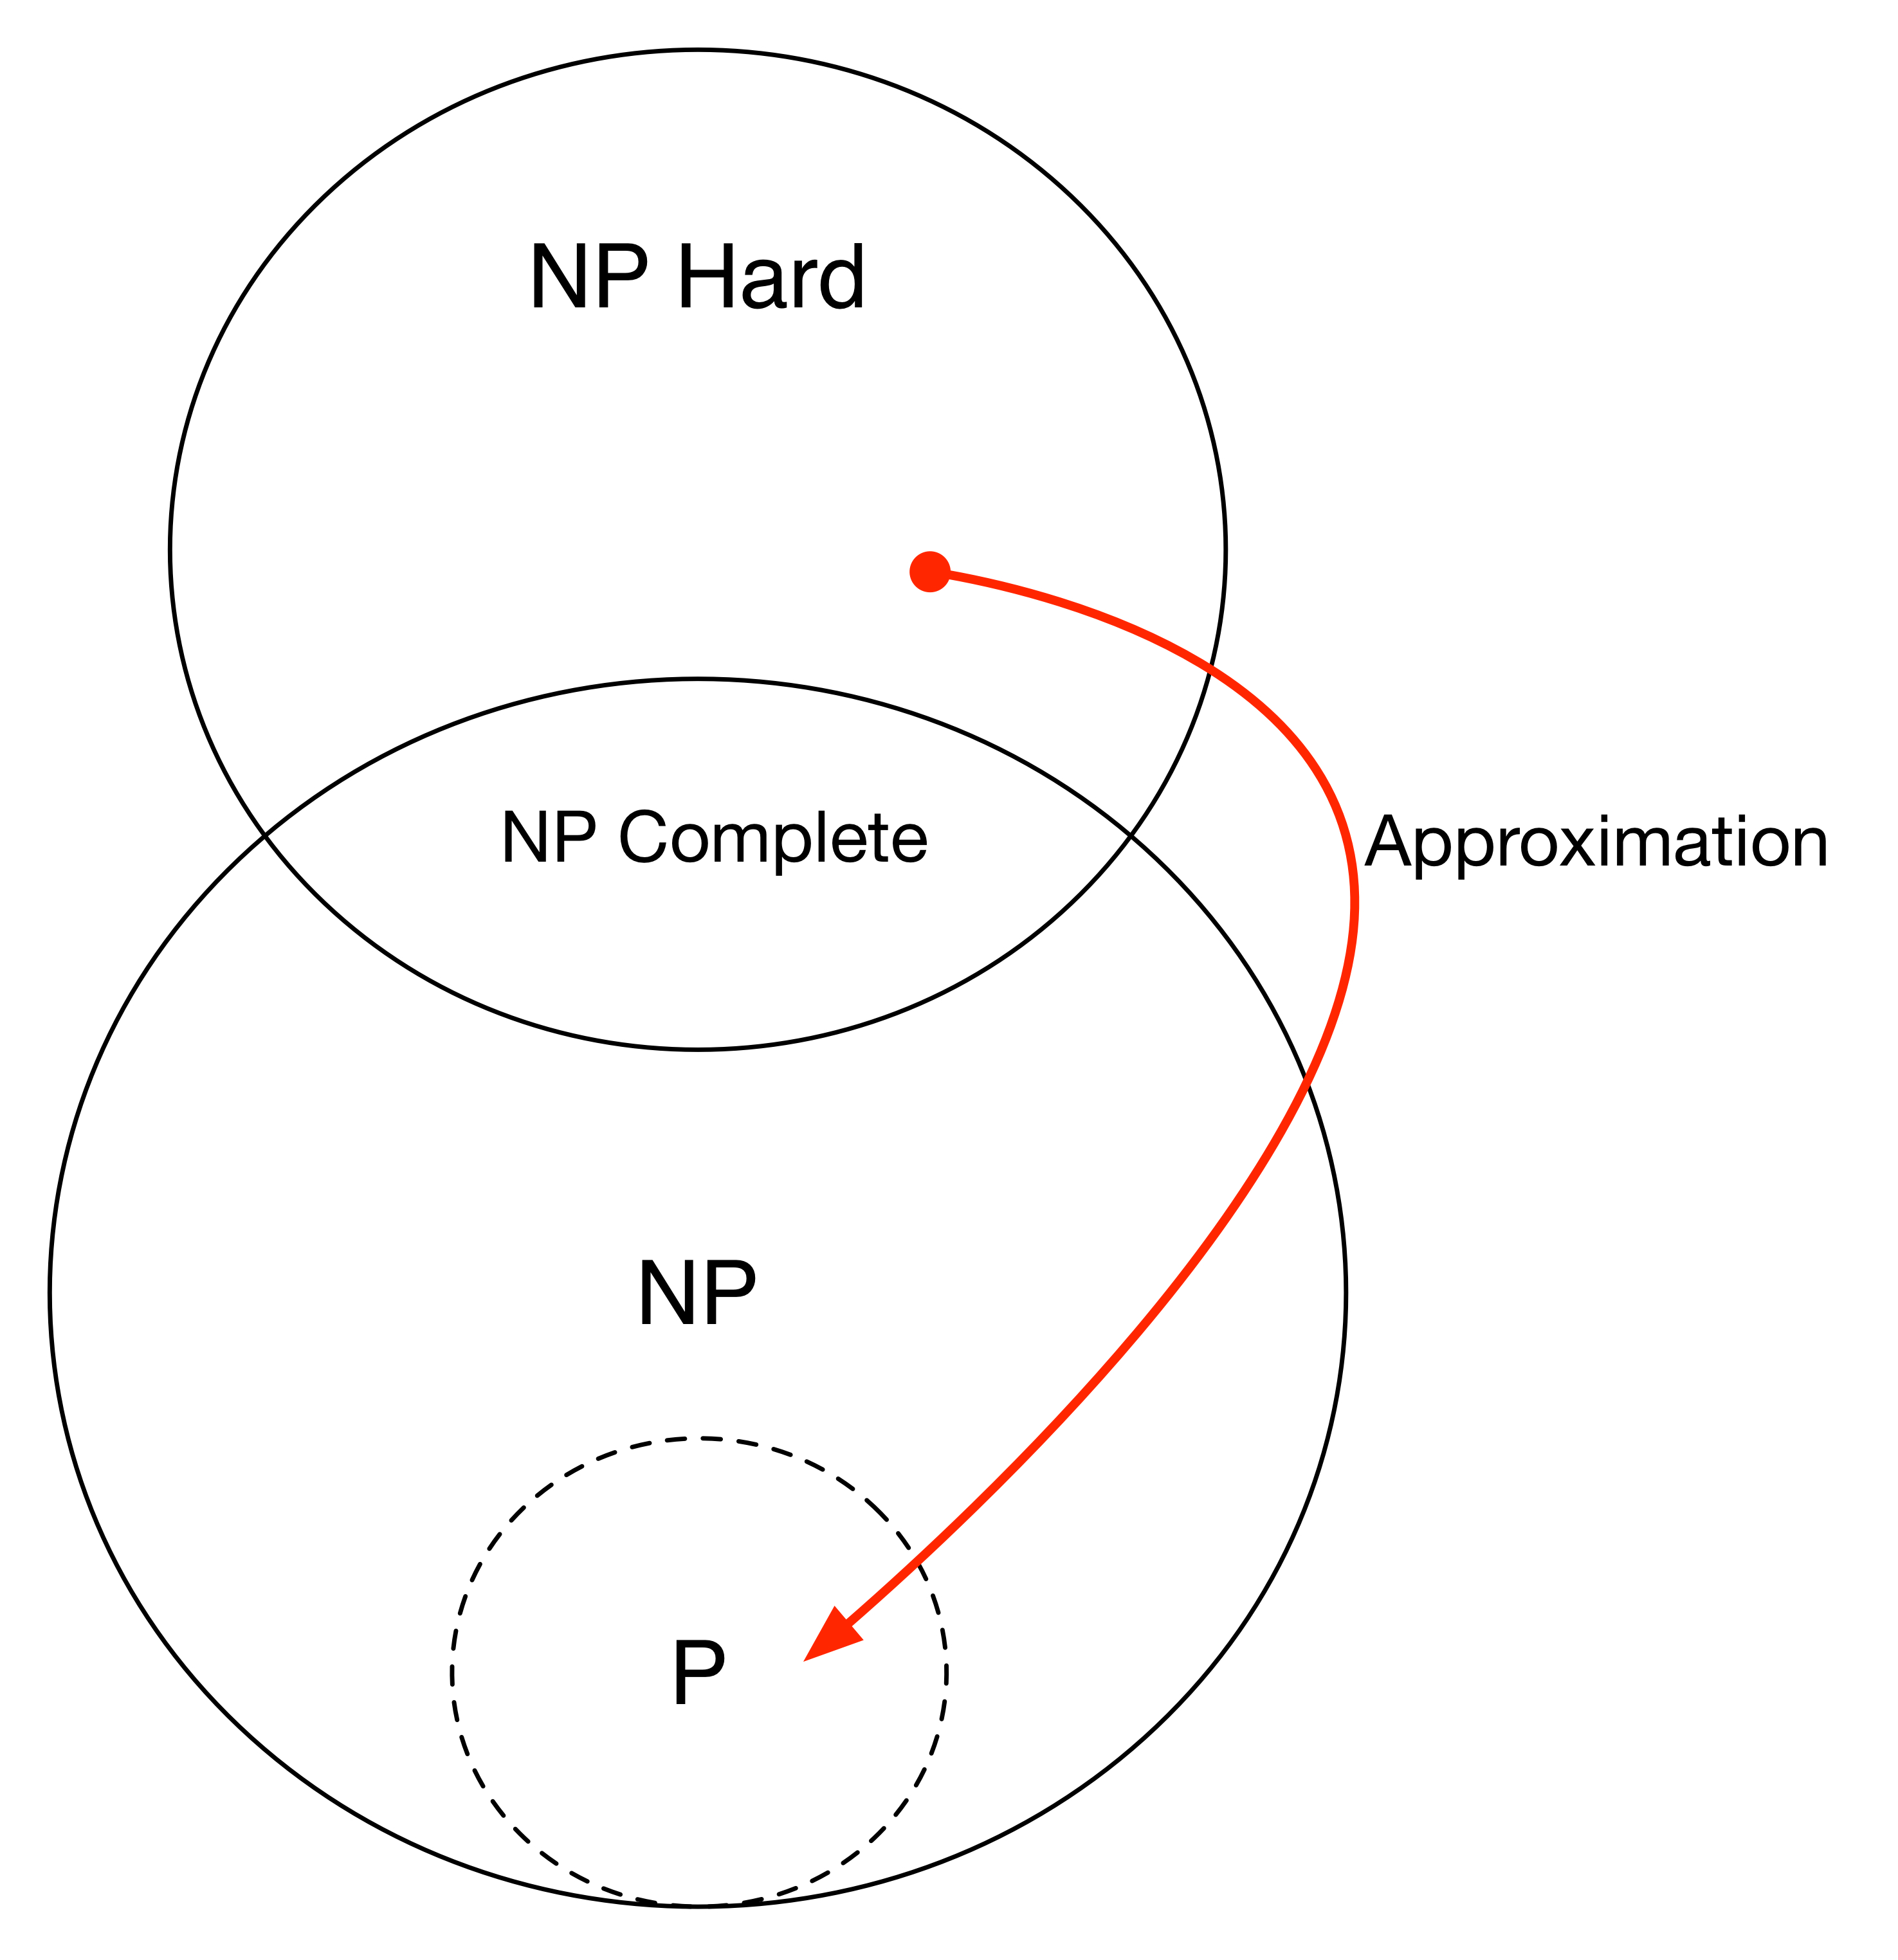
\includegraphics[scale=0.4]{figs/np_approx}
\end{columns}
\end{plain}


%-------------------------------------------------%
\section[Algorithm]{Algorithm}

\begin{plain}{Algorithm}
Input: Corpus $\mathcal{D}$, Number of topics $K$\\
\vspace{1ex}
Output: Word-topic matrix $A$, topic-topic matrix $R$\\
\begin{enumerate}
	\item Compute word-word co-occurrence matrix
	\item Normalize the matrix
	\item Find anchor words
	\item Recover topics
\end{enumerate}
\vspace{1ex}
Assumptions:
	\begin{itemize}
		\p Topics may be correlated
		\p Word-topic distributions are separable
	\end{itemize}
\end{plain}


\begin{plain}{Contributions}
\begin{enumerate}
	\p Anchor Selection
	\begin{itemize}
		\p Combinatorial rather than ILP
		\p Stable in the presence of noise
		\p polynomial sample complexity
	\end{itemize}
	
	\p Recovery step
	\begin{itemize}
		\p Previous matrix-inversion approach sensitive to noise
		\p Replaced with Gradient-based inference
	\end{itemize}
	
	\p Empirical comparison of algorithms
\end{enumerate}
\end{plain}

%-------------------------------------------------%
\section[Anchor Selection]{Efficiently Finding Anchor Words}
\begin{plain}{Word-word co-occurrence matrix}
\begin{center}
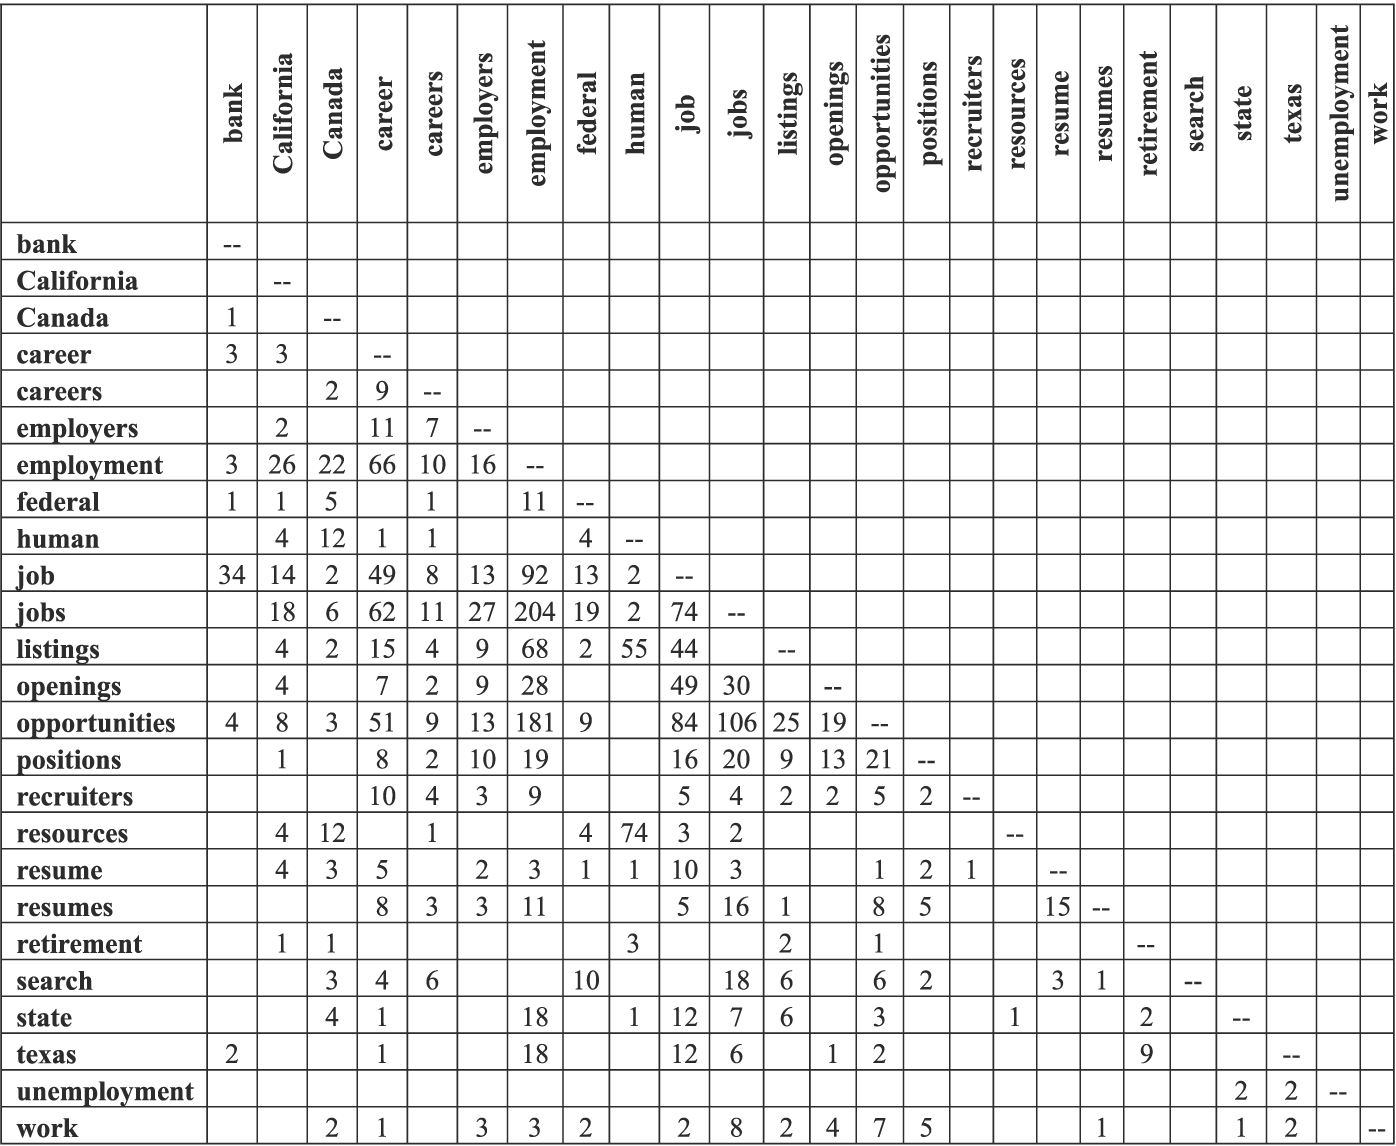
\includegraphics[scale=0.7]{figs/word_word}
\end{center}
\end{plain}

\begin{plain}{Words as vertices}
\begin{center}
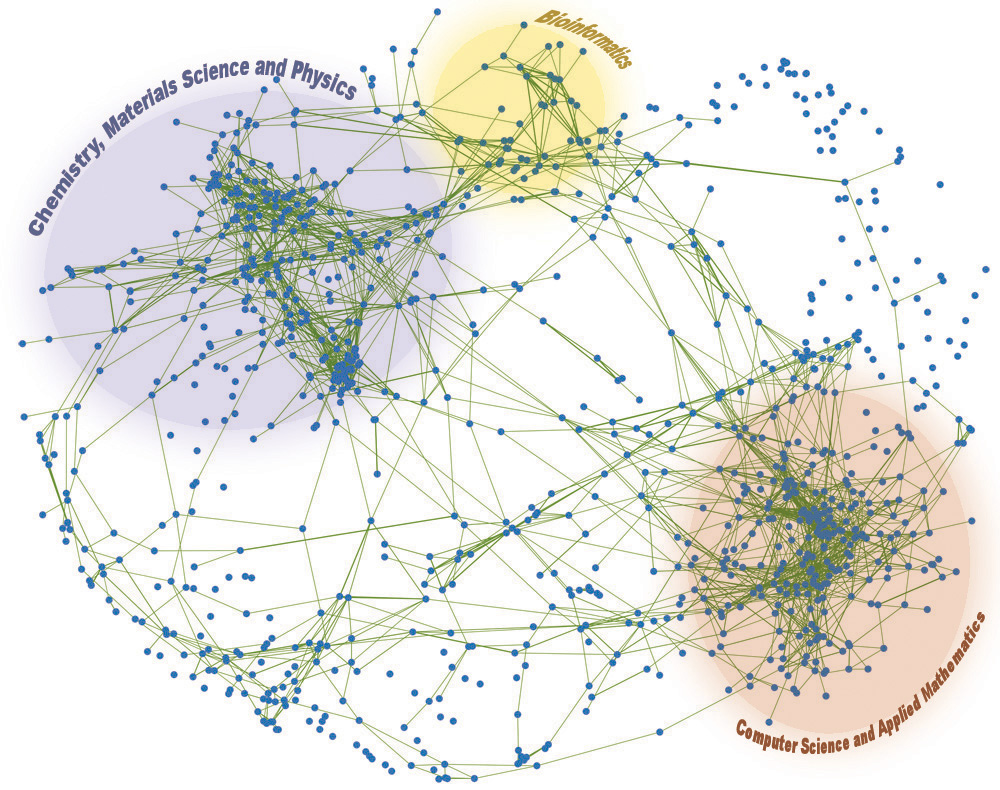
\includegraphics[scale=2.1]{figs/vertices2}
\end{center}
\end{plain}

\begin{plain}{Convex Hull}
\begin{tabular}{cc}
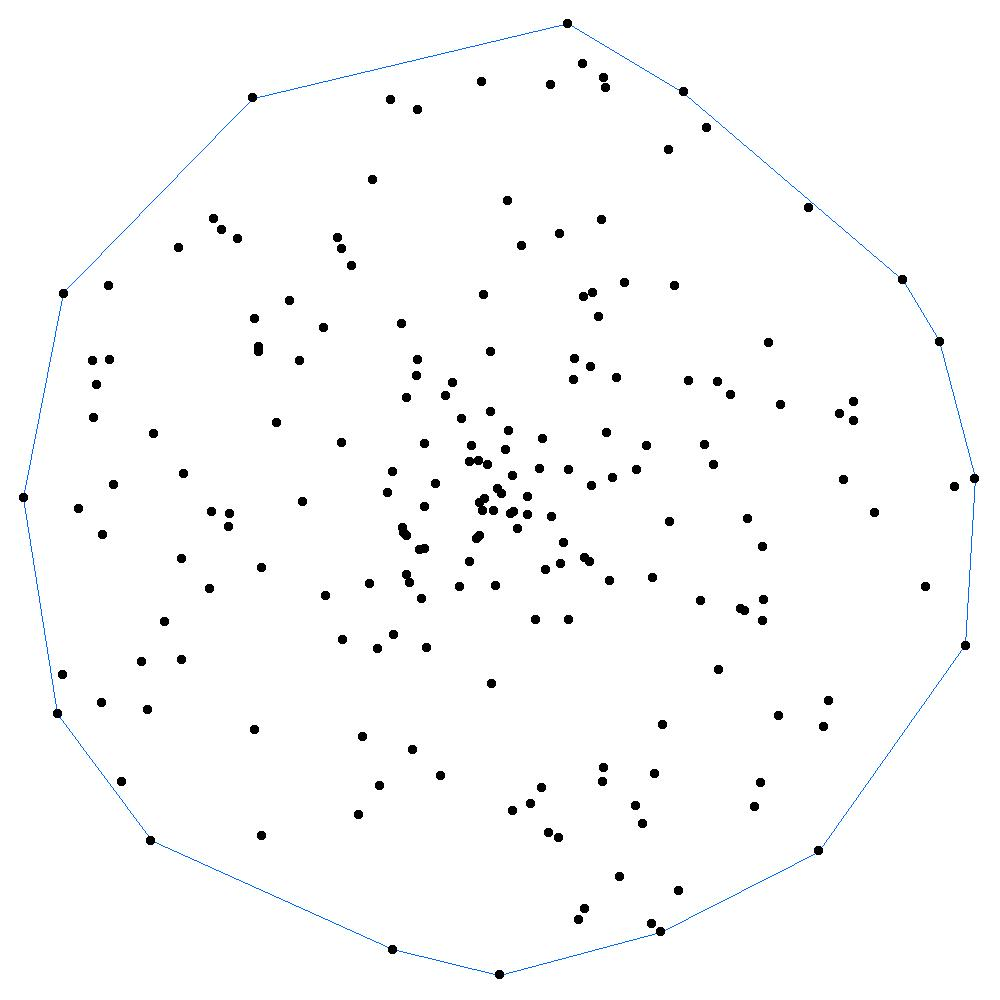
\includegraphics[scale=0.14]{figs/2d_convex_hull2} &
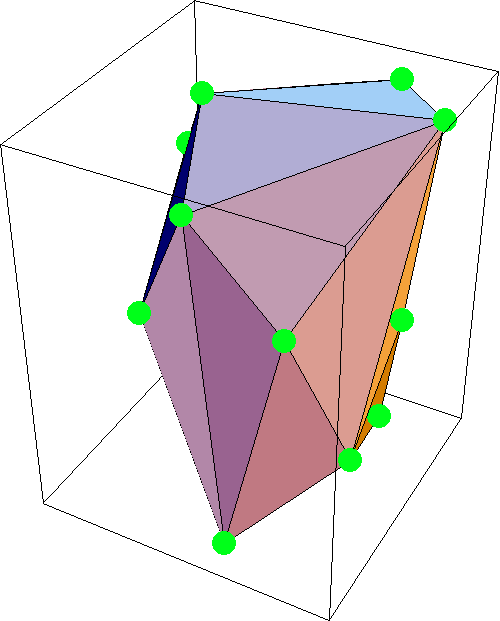
\includegraphics[scale=0.3]{figs/3d_convex_hull2}
\end{tabular}
\end{plain}

\begin{plain}{Computing Convex Hull}
\begin{itemize}
\item Efficient for 2 dimensions - O($n\log{n}$)
\item Inefficient for $n>2$ dimensions
\item Complexity depends on method and approximation used
\item Previous method: ILP
\item New method: Recursive greedy
\begin{enumerate}
\item Compute subspace span of current convex hull
\item Find point furthest from this sub-span
\item Add point to convex hull
\item Repeat until $K$ points found
\end{enumerate}
\end{itemize}
\end{plain}

%-------------------------------------------------%
\section[Topic Recovery]{Topic Recovery via Bayes' Rule}
\begin{plain}{Topic Recovery Task}
\begin{itemize}
\p Recovers the topics
\p Represented as topic-word distributions
\p Topic uniquely identified by anchor word
\end{itemize}
\end{plain}

\begin{plain}{Previous method}
\begin{enumerate}
\p Discard rows not containing anchor words from word-word co-occurrence matrix (Q)
\p Permute matrix into a diagonal matrix
\p We know that $Q=ARA^T$ where $A$ is the word-topic matrix and $R$ is the topic-topic matrix
\p Solve $Q = ARA^T$ using matrix inversion
\end{enumerate}
\end{plain}

\begin{plain}{Word-word co-occurrence probability matrix}
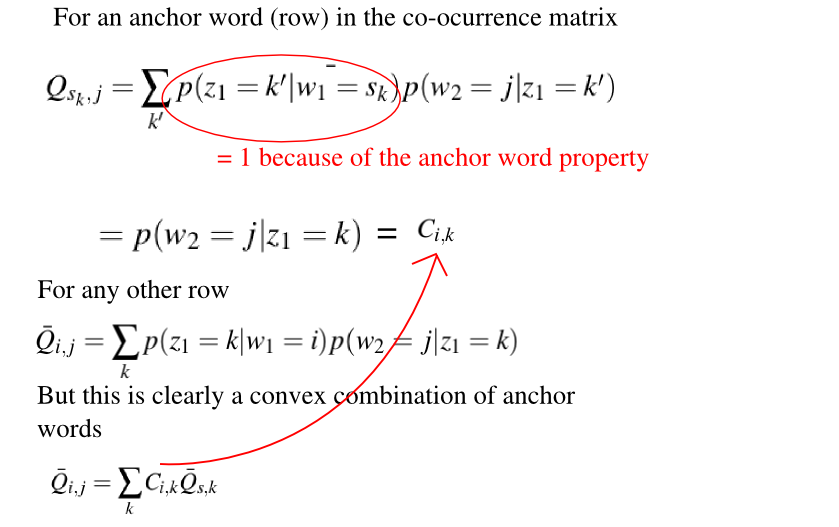
\includegraphics[scale=0.5]{figs/Q}
\end{plain}

\begin{plain}{New method}
\begin{itemize}
\p Row normalize $Q$ into $\bar{Q}$
\p Recover $A$ and $R$ using Bayes rule
\end{itemize}
$$p(w_1 = i | z_1 = k) = \frac{p(z_1 = k | w_1 = i)p(w_1 = i)}{\sum_i{p(z_1=k | w_1 = i^\prime)p(w_1=i^\prime)}}$$
\end{plain}

%-------------------------------------------------%
\section[Results]{Experimental Results}
\begin{plain}{Experiments}
\begin{center}
\hspace{-3em}
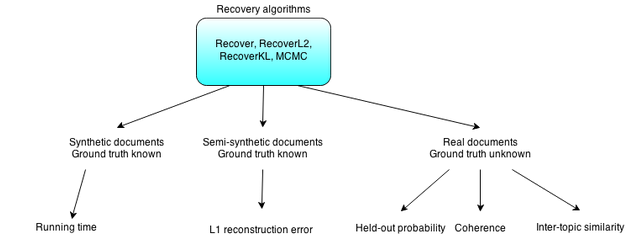
\includegraphics[scale=0.7]{figs/results_method}
\end{center}
\end{plain}

\begin{plain}{Metrics}
\begin{itemize}
\p Ground truth known
\begin{itemize}
\p Reconstruction error
\end{itemize}
\p Ground truth unknown
\begin{itemize}
\p Held out probability - probability of an unseen document under the learned model
\p Coherence - measure of semantic quality
\p Inter-topic similarity - measure of uniqueness of topics
\end{itemize}
\end{itemize}


\end{plain}

%\begin{plain}{Documents}
%TODO: Talk about semi-synthetic documents, real documents and the need for both
%\end{plain}

\begin{plain}{Results - Efficiency}
\begin{center}
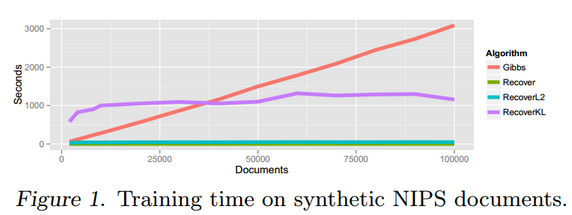
\includegraphics[scale=0.7]{figs/results_fig1}
\end{center}
\end{plain}

\begin{plain}{Results - Reconstruction error}
\begin{center}
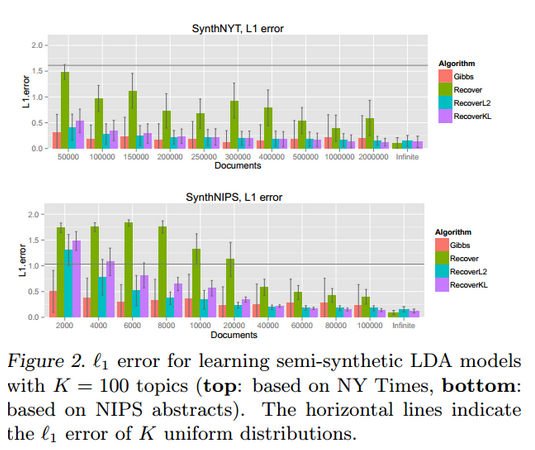
\includegraphics[scale=0.58]{figs/results_fig2}
\end{center}
\end{plain}

\begin{plain}{Results - Held out probability, coherence and unique words}
\begin{center}
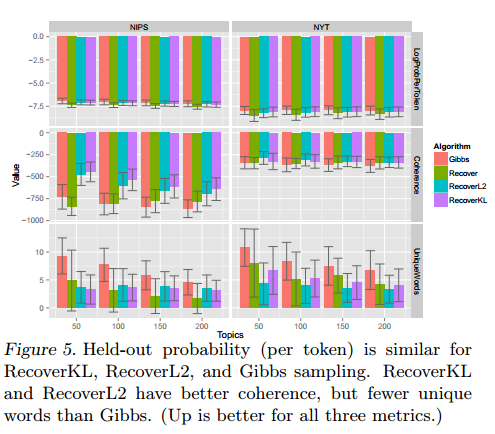
\includegraphics[scale=0.6]{figs/results_fig5}
\end{center}
\end{plain}

%-------------------------------------------------%
\section[Conclusion]{Conclusion}
\begin{plain}{Summary}
\begin{itemize}
\p New algorithms for topic recovery
	\begin{itemize}
		\p Empirical results comparable to MCMC
		\p Anchor word assumption
		\p Bayes' rule $\rightarrow$ empirical performance improvements
	\end{itemize}
\p Simple to implement, maintains provable guarantees
\p Attractive feature: \emph{Running time independent of corpus size} 
\end{itemize}
\end{plain}

\begin{plain}{Future Work}
\begin{itemize}
\p Use output of algorithms for further optimization
\p Parallel implementations
\end{itemize}
\end{plain}


\begin{plain}{Comments}
\begin{itemize}
\p Theory is consistent with results: large performance improvements
\p No obvious inconsistencies
\p Incremental contrbution
\end{itemize}
\end{plain}


\begin{plain}{}
\begin{center}
\Huge
Thanks!\\
\vspace{3ex}
\Large
Any questions please email either of us:\\
\vspace{2ex}
\large
\textbf{Vanush Vaswani}\\
\normalsize
vvas9619@uni.sydney.edu.au\\
\vspace{1ex}
\large
\textbf{Kristy Hughes}\\
\normalsize
khug2372@uni.sydney.edu.au
\end{center}
\end{plain}

\end{document}
